% Intended LaTeX compiler: pdflatex
\documentclass[10pt,a4paper,UTF8]{article}
\usepackage{zclorg}
\author{张朝龙}
\date{}
\title{对偶映射的矩阵以及矩阵的秩}
\hypersetup{
 pdfauthor={张朝龙},
 pdftitle={对偶映射的矩阵以及矩阵的秩},
 pdfkeywords={},
 pdfsubject={},
 pdfcreator={Emacs 25.0.50.1 (Org mode 9.0.5)}, 
 pdflang={English}}
\begin{document}

\maketitle
\tableofcontents
\titlepic{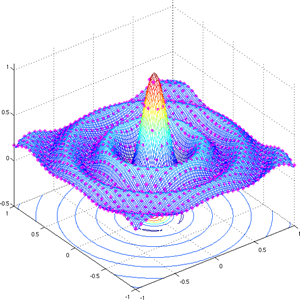
\includegraphics[scale=0.25]{../../img/sinc.PNG}}
我非常喜欢《linear algebra done right》这本书。其原因之一是这本书从头到尾都不是从矩阵到线性空间,而是从线性空间到矩阵。在 \href{matrix-for-linear-map.org}{线性映射和矩阵的关系} 一文中,我们从线性映射引出了矩阵, 这种自然的过渡不知道比从莫名其妙的行列式高明多少。说实话,大一的时候碰到行列式,然后进行各种稀奇古怪的计算时,我的内心是崩溃的,你现在还记得四阶行列式用伴随子计算的过程么?忘了最好!;好不容易从行列式出来,又突然进入了矩阵的泥潭,这完全是再次莫名其妙,等到线性映射出现的时候,已经“三而竭”了。尽管最后考了高分,那完全是填鸭式突击的结果。

在本文我们再次把矩阵和线性映射紧密联系。这次我们先给出矩阵转置的定义,然后论述矩阵的转置是如何和线性空间以及线性映射结合的。

\section{对偶映射的矩阵}
\label{sec:org1a17dc2}

\begin{definition}
矩阵\(A\)的转置是通过互换\(A\)的行和列来完成的。确切的说,若\(A\)是\(m\times n\)的矩阵,则\(A^{t}\)是\(n\times m\)矩阵,其元素由下面的等式给出:
\[(A^{t})_{k,j} = A_{j,k}\]
\end{definition}

转置有一个特别好的性质:对所有的\(m\times n\)矩阵\(A,C\)和所有\(\lambda\in \mathbf{F}\)均有\((A+C)^{t} A^{t} + C^{t}\) 且\((\lambda A)^{t} = \lambda A^{t}\)。

\begin{theorem}
若\(A\)是\(m\times n\)矩阵,\(C\)是\(n\times p\)矩阵,则:\[(AC)^{t} = C^{t}A^{t}\]
\end{theorem}

\begin{proof}
设\(1\leq k \leq m, 1\leq j\leq p\),则:
\begin{eqnarray}
\label{eq:1}
(AC)^{t}_{j,k}&=& (AC)_{k,j} \\
&=&\sum_{r=1}^{n}A_{k,r}C_{r,j} \\
&=&\sum_{r=1}^{n}(A^{t})_{r,k}(C^{t})_{j,r} \\
&=&\sum_{r=1}^{n} (C^{t})_{j,r}(A^{t})_{r,k} \\
&=& (C^{t}A^{t})_{j,k}
\end{eqnarray}

即:\((AC)^{t} = C^{t}A^{t}\)
\end{proof}

\begin{theorem}
假设\(V\)有基\(v_{1},\ldots ,v_{n}\),\(V^{'}\)的对偶基\(\varphi_{1},\ldots ,\varphi_{n}\),并假设\(W\)有基\(w_{1},\ldots ,w_{m}\)以及\(W^{'}\)的对偶基\(\psi_{1},\ldots ,\psi_{m}\),于是\(\mathcal{M}(T)\)是按\(V\)和\(W\)的上述基对应的矩阵,\(\mathcal{M}(T^{'})\)时按照\(W^{'}\)和\(V^{'}\)对应的矩阵计算。

则有对于\(T\in \mathcal{L}(V,W)\),有\(\mathcal{M}(T^{'}) = (\mathcal{M}(T))^{t}\)
\end{theorem}

\begin{proof}
这个命题的证明仅仅需要紧扣定义。

设\(A = \mathcal{M}(T)\),\(C = \mathcal{M}(T^{'})\),再设\(1\leq j \leq m\),\(1\leq k \leq n\),由\(\mathcal{M}(T^{'})\)的定义我们有:
\begin{eqnarray}
\label{eq:2}
T^{'}(\psi_{j})&=& \sum_{r=1}^{n}C_{r,j}\varphi_{r} 
\end{eqnarray}
因为\(T^{'}(\psi_{j}) = \psi_{j} \circ T\) ,所以,将上式两端作用到\(v_{k}\)上,有:
\begin{eqnarray}
\label{eq:3}
(\psi_{j}\circ T)(v_{k})&=& \sum_{r=1}^{n}C_{r,j}\varphi_{r}(k) \\
&=&C_{k,j}
\end{eqnarray}
另外,根据\(T(v_{k})\)的定义我们有:
\begin{eqnarray}
\label{eq:4}
(\psi_{j}\circ T)(v_{k})&=& \psi_{j}(Tv_{k}) \\
&=& \psi_{j}(\sum_{r=1}^{m} A_{r,k}w_{r}) \\
&=&\sum_{r=1}^{m}A_{r,k}\psi_{j}(w_{r}) \\
&=&A_{j,k}
\end{eqnarray}

综上有:\(A_{j,k} = C_{k,j}\),即\(A = C^{t}\)
\end{proof}
\section{矩阵的秩}
\label{sec:org1dbac4b}


\begin{definition}
设\(A\)是元素属于\(F\)的\(m\times n\)矩阵:
\begin{enumerate}
\item \(A\)的行秩是\(A\)的诸行在\(\mathbf{F}^{1,n}\)中的张成空间的维数;
\item \(A\)的列秩是\(A\)的诸列在\(\mathbf{F}^{m,1}\)中的张成空间的维数。
\end{enumerate}
\end{definition}

\begin{theorem}
设\(V\)和\(W\)都是有限维的,\(T\in \mathcal{L}(V,W)\),则\(\dim range T\)等于\(\mathcal{M}(T)\)的列秩。
\end{theorem}

\begin{proof}
设\(v_{1},\ldots ,v_{n}\)是\(V\)的基,\(w_{1},\ldots ,w_{n}\)是\(W\)的基。则将\(w\in span(Tv_{1},\ldots ,Tv_{n})\)变为\(\mathcal{M}(w)\)的函数是从\(span(Tv_{1},\ldots ,Tv_{n})\)到\(span(\mathcal{M}(Tv_{1}), \ldots ,\mathcal{M}(Tv_{n}))\)的同构。于是\(\dim span(Tv_{1},\ldots ,Tv_{n}) = \dim span(\mathcal{M}(Tv_{1}), \mathcal{M}(Tv_{n}))\) 等式右边的维数等于\(\mathcal{M}(T)\)的列秩。

因为\(rangeT = span(Tv_{1},\ldots ,Tv_{n})\),所以\(\dim rangeT = \dim span(Tv_{1},\ldots ,Tv_{n})\)
\end{proof}
\begin{theorem}
设\(A \in \mathbf{F}^{m,n}\),则\(A\)的行秩等于\(A\)的列秩。
\end{theorem}
\end{document}
